\documentclass[12pt,a4paper, hidelinks]{article}
\usepackage[utf8]{inputenc}
\usepackage{amsmath}
\usepackage{amsfonts}
\usepackage{amssymb}
\usepackage{amsthm}
\usepackage{graphicx}
\usepackage{hyperref}
\usepackage{geometry}
\geometry{a4paper, margin=1in}
\usepackage{fancyhdr}
\usepackage{indentfirst} % Add this line to enable first paragraph indentation
\usepackage{times} % Use Times New Roman font
\usepackage{setspace}
\usepackage{graphicx}
\usepackage{float}
\usepackage{listings}
\usepackage{tabularx}

\setstretch{1.15} % Adjust the stretch factor as needed

\pagestyle{fancy}
\fancyhf{}  % Clear header and footer fields
\rfoot{\thepage}  % Place page number at the right bottom corner
\renewcommand{\headrulewidth}{0pt}  % Remove the header line





\begin{document}

% Title Page
\begin{titlepage}
    \centering
    \vspace*{0.5 cm}
    
\includegraphics[width=0.20\textwidth]{images/logo.png}\par\vspace{1cm}
    {\scshape\LARGE Warsaw University of Technology \par}
    \vspace{1cm}
    {\scshape\Large Faculty of Mathematics and Information Science\par}
    \vspace{1.5cm}
    {\huge\bfseries Real-time fraudulent transactions detection \par}
    \vspace{1cm}
    {\Large\itshape Big Data Analytics\par}
    \vfill
    % \vspace{2cm}
    \begin{flushright}

    {\Large\textbf Salveen Singh Dutt (317298) \\ Karina Tiurina (335943)  \\ Patryk Prusak (305794) \par}
    \vfill
    {Supervisor\par}
    {\Large mgr inz. Jakub Abelski \par}
    
    \end{flushright}
    \vfill
    % \break
    {\large Warsaw 2025\par}
    \vspace{1cm}
\end{titlepage}

\newpage

% Table of contents
\tableofcontents
\newpage % Optional: Add a page break after the TOC

\section*{Introduction}
\addcontentsline{toc}{section}{Introduction}

This project aims to plan and implement a financial transaction processing system that identifies suspicious and fraudulent activity in real time. Given the enormous volume of incoming data, the project utilizes big data technologies and advanced machine learning algorithms for anomaly detection. The project is available on the GitHub repository: \href{https://github.com/salveendutt/Big-Data-Analytics}{https://github.com/salveendutt/Big-Data-Analytics}.

\subsection*{Updates from Milestone 3}
\addcontentsline{toc}{subsection}{Updates from Milestone 3}
The serving layer has been introduced with Apache Superset and TrinoDB. The initial model is now being trained locally with Spark.



\section{High level description}

The main idea is to implement automatic transaction processing so that the transaction is blocked for further manual review when a fraudulent activity occurs. The aim is to reduce the end-users financial losses and enhance online payment security, ensuring a safer experience for all customers.

The project's main end-users are financial institutions (we will call them 'Managers') and their customers who are executing the payments. Although both categories can benefit from the solution, in our implementation, we will mainly focus on Managers to limit additional data in storage.

The list below contains the main features that we expect to implement for Managers:
\begin{enumerate}
    \item Fraudulent transactions are automatically highlighted so that it is easier to identify suspicious activity;
    \item The history of transactions is stored and available for later review;
    \item A dashboard with statistics of fraudulent activity is available and customizable for better localization of issues (e.g., too large amount, unusual location);
    \item Anomaly-detection model is continuously updated so that fraud detection utilizes new historical data and is more accurate on future transactions;
    \item Data streaming processing and batch jobs are customizable so that the testing of the model's performance is simplified.
\end{enumerate}


\newpage

\section{Data sources}

Due to strict security regulations on personal and financial data, finding open-source actual transaction data for model training and streaming is challenging. Therefore, available synthetic and anonymized datasets will be used. The table below contains a description of the data sources. Each data source is described in more detail in the dedicated subsections.

\begin{table}[h!]
\centering


\begin{tabular}{|p{4.8cm}|p{3.5cm}|p{2cm}|p{2cm}|p{1.5cm}|}
\hline
\textbf{Data Source} & \textbf{Content} & \textbf{Volume} &  \textbf{Fraud, \%} & \textbf{Link} \\
\hline
1. Fraudulent Transactions Data &  Dataset for predicting fraudulent transactions for a financial company. &  6,362,620 rows and 10 columns (493.53 MB) & 0.13\% & \href{https://www.kaggle.com/datasets/chitwanmanchanda/fraudulent-transactions-data}{Kaggle} \\
\hline
2. Credit Card Fraud & Contains features with transactional context. & 1,000,000 transactions (58.9 MB) & 8.7\% & \href{https://www.openml.org/search?type=data\&status=active\&id=45955}{OpenML} \\
\hline
3. Credit Card Transactions Synthetic Data Generation & A collection of synthetic credit card transaction data. & 1,785,308 transactions; 5,000 customers; (153.66 MB) & 3\% & \href{https://www.kaggle.com/datasets/cgrodrigues/credit-card-transactions-synthetic-data-generation?select=transactions_df.csv}{Kaggle} \\
\hline
4. Credit Card Fraud Detection & Transactions made by credit cards in September 2013 by European cardholders. & 284,807 transactions (150.83 MB) & 0.17\% & \href{https://www.kaggle.com/datasets/mlg-ulb/creditcardfraud}{Kaggle} \\
\hline
\end{tabular}

\caption{Data sources}
\end{table}

\begin{figure}[h!]
    \centering
    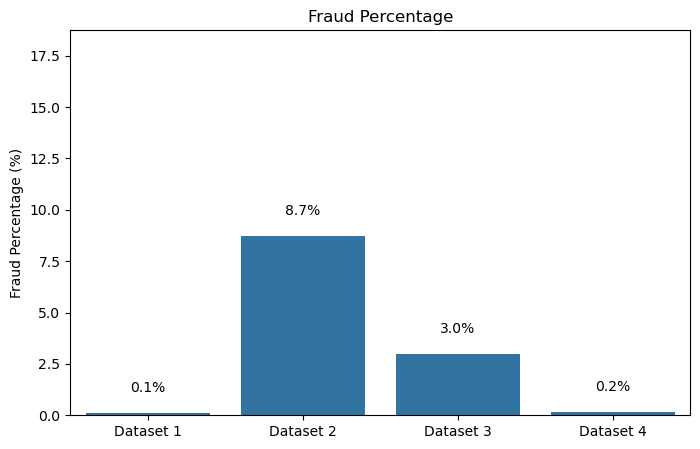
\includegraphics[width=0.7\textwidth]{images/fraud-distribution.png}
    \caption{Fraud distribution across datasets}
    \label{fig:fraudDistribution}
\end{figure}

Data-streaming API was implemented from scratch. The assumption was that it would use the above datasets; with a specified time frame, it would choose a random transaction not used for training and push it for further processing. The probability of a fraudulent transaction will be set manually to some high enough constant value for testing purposes. A detailed description of the implemented streaming API can be found in Chapter 3.

The content of the datasets is exceptionally different, which makes it impossible to combine them into a single dataset. Therefore, each dataset will be treated separately for streaming and ML training.

Complete Exploratory Data Analysis can be found in the 'eda' subfolder of our repository. In the report we included fraud distribution and the amount distribution for each dataset where applicable.


\subsection{Fraudulent Transactions Data (Kaggle)}

The dataset contains transactions for a financial company, indicating whether they are fraudulent. Data for the case is available in CSV format, which has 6362620 rows and ten columns. The entire column description is presented in Table 2.

\begin{table}[ht!]
\centering
\begin{tabular}{|p{3cm}|p{9.8cm}|p{2cm}|}
\hline
\textbf{Column} & \textbf{Content} & \textbf{Type} \\
\hline
step & maps a unit of time in the real world. In this case, 1 step is 1 hour. Total steps 744 (30 days simulation) & int \\
\hline
type & type of the transaction. Available values: CASH-IN, CASH-OUT, DEBIT, PAYMENT, and TRANSFER & str \\
\hline
amount & amount of the transaction in local currency & float \\
\hline
nameOrig & customer who started the transaction & str \\
\hline
oldbalanceOrg & initial balance before the transaction & float \\
\hline
newbalanceOrig & new balance after the transaction & float \\
\hline
nameDest & customer who is the recipient of the transaction & str \\
\hline
oldbalanceDest & initial balance recipient before the transaction. Note that there is no information for customers that start with M (Merchants) & float \\
\hline
newbalanceDest & new balance recipient after the transaction. Note that there is no information for customers that start with M (Merchants) & float \\
\hline
isFraud & these are the transactions made by the fraudulent agents inside the simulation. In this specific dataset, the fraudulent behavior of the agents aims to profit by taking control of customers' accounts and trying to empty the funds by transferring them to another account and then cashing out of the system & int \\
\hline
isFlaggedFraud & the business model aims to control massive transfers from one account to another and flags illegal attempts. An illegal attempt in this dataset is an attempt to transfer more than 200.000 in a single transaction & int \\
\hline
\end{tabular}
\caption{Columns description. Dataset 1: 'Fraudulent Transactions Data' from Kaggle}
\end{table}

The following transformation should be done to pass the dataset to the ML models:
\begin{enumerate}
    \item 'type' column values CASH-IN, CASH-OUT, DEBIT, PAYMENT, and TRANSFER transformed to 1, 2, 3, 4, and 5, respectively;
    \item a new attribute 'isMerchant' is calculated. 1 if 'nameDest' starts with 'M', 0 - otherwise.
\end{enumerate}

Generally, the dataset and clean and structured, no other preprocessing, except for the described above is necessary. The potential issue is that it is highly unbalanced (less than 1\% of fraud transactions) and contains quite a small number of features (6) for model training. 

\begin{figure}[h!]
    \centering
    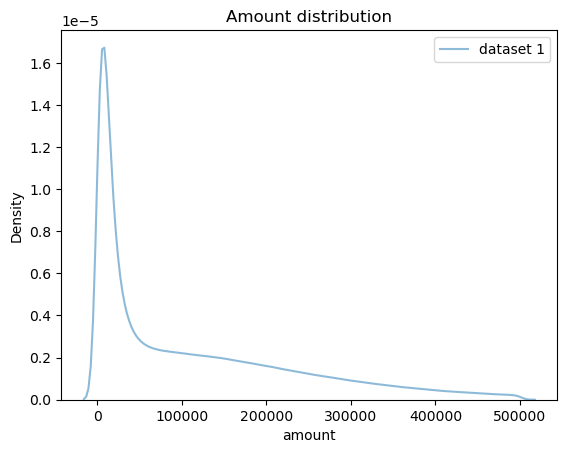
\includegraphics[width=0.7\textwidth]{images/amount1.png}
    \caption{Amount distribution of dataset 1}
    \label{fig:amount1}
\end{figure}


\subsection{Credit Card Fraud (OpenML)}

This dataset captures transaction patterns and behaviors that could indicate potential fraud in card transactions. The data comprises several features that reflect the transactional context, such as geographical location, transaction medium, and spending behavior relative to the user's history.

\begin{table}[ht!]
    \centering
    \begin{tabular}{|p{5.5cm}|p{7cm}|p{2cm}|}
    \hline
    \textbf{Column} & \textbf{Content} & \textbf{Type} \\
    \hline
    distance\_from\_home & This is a numerical feature representing the geographical distance in kilometers between the transaction location and the cardholder's home address. & float \\
    \hline
    distance\_from\_last\_transaction & This numerical attribute measures the distance in kilometers from the location of the last transaction to the current transaction location. & float \\
    \hline
    ratio\_to\_median\_purchase\_price & A numeric ratio that compares the transaction's price to the median purchase price of the user's transaction history. & float \\
    \hline
    repeat\_retailer & A binary attribute where '1' signifies that the transaction was conducted at a retailer previously used by the cardholder, and '0' indicates a new retailer. & [0, 1] \\
    \hline
    used\_chip & This binary feature indicates whether the transaction was made using a chip (1) or not (0). & [0, 1] \\
    \hline
    used\_pin\_number &  Another binary feature, where '1' signifies the use of a PIN number for the transaction, and '0' shows no PIN number was used. & [0, 1] \\
    \hline
    online\_order & This attribute identifies whether the purchase was made online ('1') or offline ('0'). & [0, 1] \\
    \hline
    fraud & A binary target variable indicating whether the transaction was fraudulent ('1') or not ('0'). & [0, 1] \\
    \hline
    \end{tabular}
    \caption{Columns description. Dataset 2: 'Credit\_Card\_Fraud\_' from OpenML}
\end{table}

The whole dataset is in the numeric form. Therefore, no additional preprocessing is necessary. The only transformation is to rename the target variable to 'isFraud' to match the format of other datasets.
The target feature balance is much better than the previous dataset: 8.7\% of fraud. An additional complication is that the feature 'amount' is not available. A ratio to the median purchase of the same customer is provided instead.

\begin{figure}[h!]
    \centering
    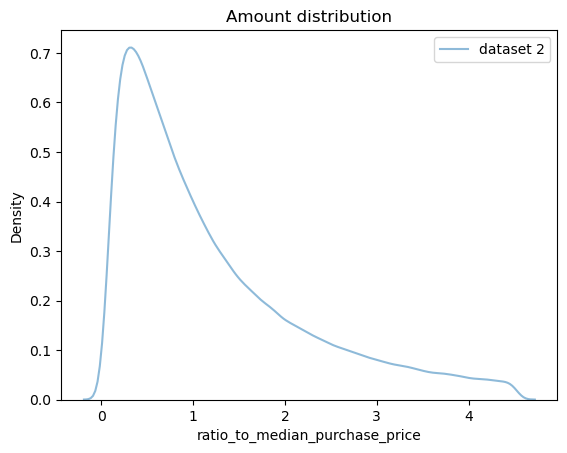
\includegraphics[width=0.7\textwidth]{images/amount2.png}
    \caption{Amount distribution of dataset 2}
    \label{fig:amount2}
\end{figure}

\subsection{Credit Card Transactions Synthetic Data Generation (Kaggle)}

This dataset is a collection of synthetic credit card transaction data. The data is designed to mimic the characteristics of actual credit card transactions while ensuring privacy and compliance with data protection regulations such as the General Data Protection Regulation (GDPR). It contains 1,785,308 transactions for 5000 customers.

\begin{table}[ht!]
    \centering
    \begin{tabular}{|p{4.5cm}|p{8cm}|p{2cm}|}
    \hline
    \textbf{Column} & \textbf{Content} & \textbf{Type} \\
    \hline
    transaction\_id & Random string containing specific transactions id & str \\
    \hline
    post\_ts & Date and time of the transaction & str \\
    \hline
    customer\_id & Specific customer id & str \\
    \hline
    bin & Bank Identification Number & int \\
    \hline
    terminal\_id & Specific terminal id & int \\
    \hline
    amt & Transaction amount & float \\
    \hline
    entry\_mode & Mode of the transaction. Possible values are Contactless, Chip, and Swipe. & str \\
    \hline 
    fraud & Target variable containing 1 for the fraudulent transaction and 0 otherwise & int \\
    \hline
    fraud\_scenario & Additional label for the transaction. 97\% of the dataset has a value of 0. No specific description for each scenario is provided.  & int, [0, 1, 2] \\
    \hline
    mean\_amount & Average transaction amount for a specific customer  & float \\
    \hline
    std\_amount & Standard deviation of the transaction amount for a specific customer  & float \\
    \hline
    mean\_nb\_tx\_per\_day & Mean number of transactions per day for a specific customer & float \\
    \hline
    customer\_bin & Bank Identification Number of a customer & int \\
    \hline
    \end{tabular}
    \caption{Columns description. Dataset 3: 'Credit Card Transactions Synthetic Data Generation' from Kaggle}
\end{table}

Like other datasets, it is quite unbalanced, with 3\% of fraudulent transactions. The following preprocessing should be done before passing rows to the ML task:
\begin{enumerate}
    \item 'entry\_mode' column values Contactless, Chip, and Swipe transformed to 1, 2, and 3, respectively;
    \item 'amt' renamed to 'amount',
    \item 'fraud' renamed to 'isFraud',
    \item transaction data itself contains only customer ID. Therefore, an additional step is to find the customer and add related features to the output.
\end{enumerate}

\begin{figure}[h!]
    \centering
    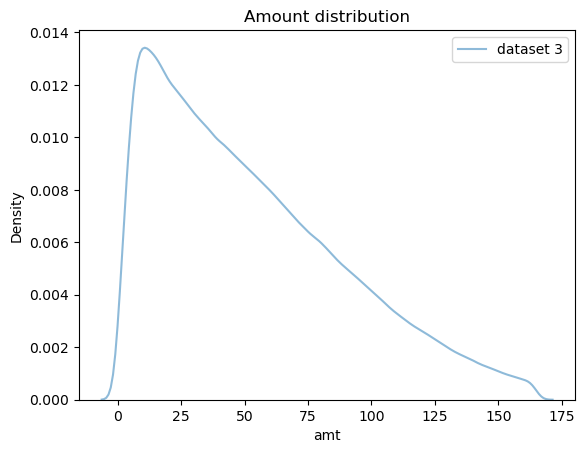
\includegraphics[width=0.7\textwidth]{images/amount3.png}
    \caption{Amount distribution of dataset 3}
    \label{fig:amount3}
\end{figure}

\subsection{Credit Card Fraud Detection (Kaggle)}

The dataset contains transactions made by credit cards in September 2013 by European cardholders. It includes 284,807 transactions, with only 492 (less than 1\%) of fraud ones. Due to confidentiality issues, the dataset contains only numerical input variables resulting from a PCA transformation.

\begin{table}[ht!]
    \centering
    \begin{tabular}{|p{2.5cm}|p{10cm}|p{2cm}|}
    \hline
    \textbf{Column} & \textbf{Content} & \textbf{Type} \\
    \hline
    Time & The seconds elapsed between the transaction and the first transaction in the dataset & int \\
    \hline
    V1 ... V28 & The principal components obtained with PCA. The original features and more background information about the data are not provided. & float \\
    \hline
    Amount & Transaction amount & float \\
    \hline
    Class & Target variable; 1 for fraudulent transaction and 0 otherwise & int, [0, 1] \\
    \hline
    \end{tabular}
    \caption{Columns description. Dataset 4: 'Credit Card Fraud Detection' from Kaggle}
\end{table}

This dataset contains a relatively small amount of data compared to others (about 280k transactions). Therefore, we plan to keep it as an additional dataset in case of any issues with others.

Since the data has already been processed, the only necessary transormation is to rename columns 'Amount' and 'Class' to 'amount', 'isFraud' respectively.

\newpage

\section{Data acquisition strategy}

Due to the lack of publicly available open streaming APIs, we designed and implemented a custom streaming API for real-time fraud detection. Stream API is connected to the NiFi for further data collection and preprocessing. The following technological stack is used for the data acquisition:

\begin{enumerate}
    \item Python,
    \item Flask  - for the stream API,
    \item Apache NiFi - for the data collection,
    \item Docker - for deployment,
    \item Apache Kafka - for the data streaming,
    \item Kafdrop - for Kafka monitoring,
    \item Apache HDFS and Hive - as a main storage solution
    \item Zookeeper.
\end{enumerate}

When the server is started, stream API is available on localhost:5001/data/:dataset\_id. Data frequency is configurable on the NiFi side and, at the moment, is set to 1 row per 2 seconds for each dataset. The format of each incoming transaction is JSON, containing attributes as described for each dataset in Chapter 2. The streaming API randomly (10\%) returns a 500 error to simulate real-world conditions. Example screenshots of the data stream and NiFi are provided in the SKaMP\_Tests.pdf file.

Below, we present the NiFi flows for the data acquisition. Processor failures are retried 10 times, and errors are logged with the LogMessage processor with a level of 'error.' The first flow is the overview of the whole process. The three processor groups are responsible for fetching and processing the data. Inside each of the processor groups, there are:
\begin{itemize}
    \item InvokeHTTP - to fetch the data from the stream API,
    \item EvaluateJsonPath - to evaluate whether any data is missing,
    \item ReplaceText - to add year, month, and day that is used for data partitioning in Hive,
    \item PublishKafkaRecord - to send the data to Kafka,
    \item JoltTransformJSON - to preprocess the data into desired format,
    \item UpdateAttribute - to add the hdfs path attribute to the data that depends on the year, month, and day,
    \item ConvertRecord - to convert the data to the Parquet format,
    \item LogMessage - to log the errors,
    \item PutHDFS - to store the data in HDFS.
\end{itemize}


\begin{figure}[h!]
    \centering
    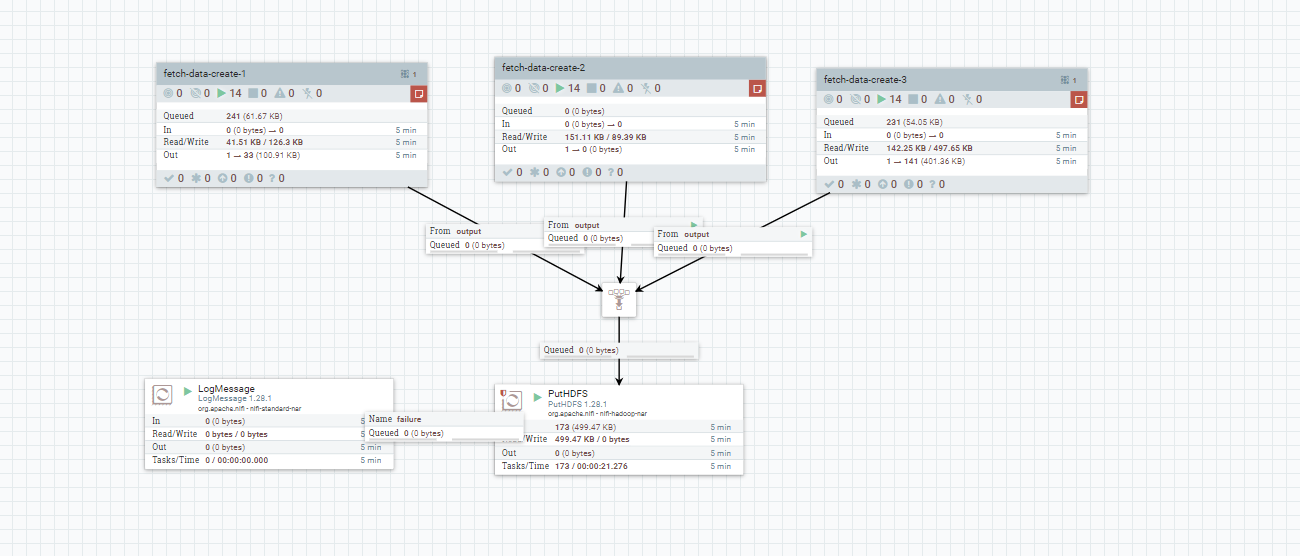
\includegraphics[width=0.95\textwidth]{images/m3-nifi-main-view.png}
    \caption{NiFi flow for the data acquisition}
    \label{fig:nifi1}
\end{figure}
\begin{figure}[h!]
    \centering
    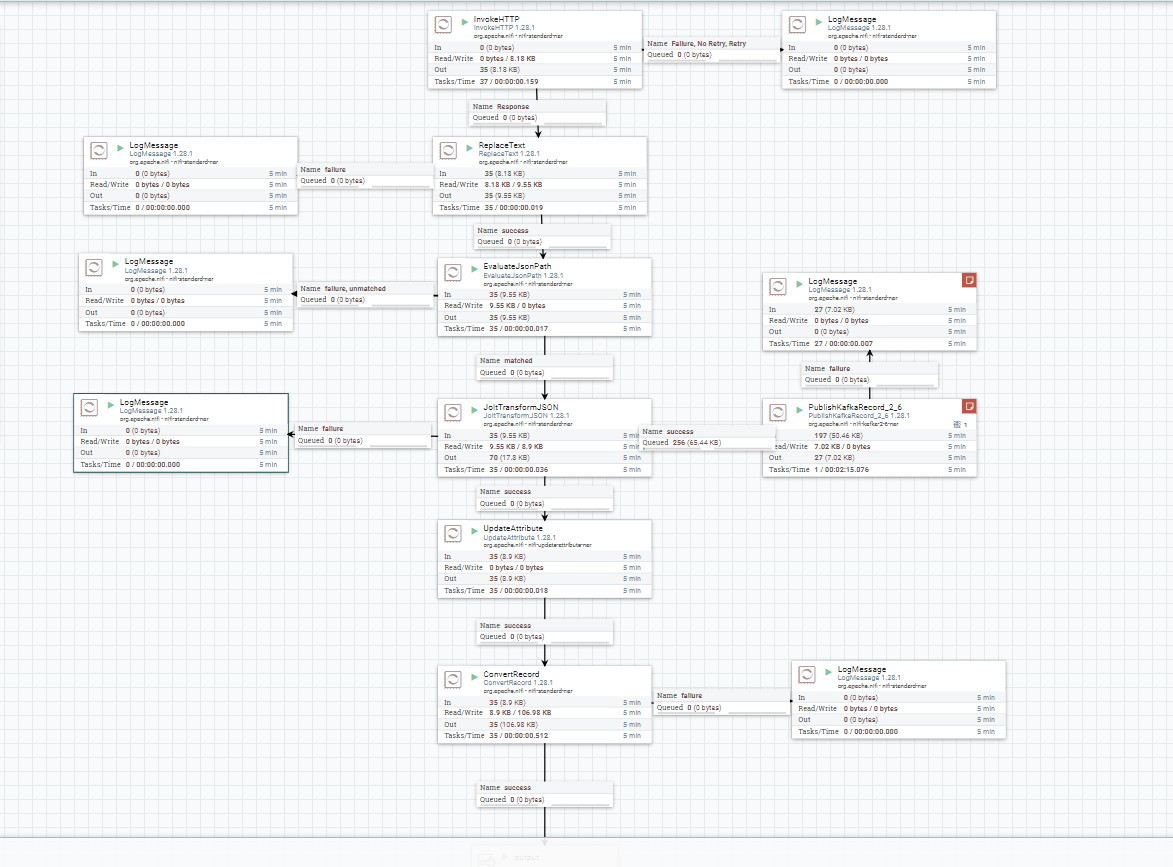
\includegraphics[width=0.95\textwidth]{images/m3-nifi-processor.png}
    \caption{Data processing flow in NiFi}
    \label{fig:nifi2}
\end{figure}
\section{Data storage strategy}

Our input data consists of structured data; there is no need to store particular data types, such as images, text files, audio, etc. Therefore, we decided to utilize an SQL-like (CQL) data warehouse system that enables analytics at a massive scale - Apache Hive.

As described in Chapter 2, our datasets contain entirely different sets of features, which makes it impossible to combine them in a single table. All incoming transactions are divided into four groups for each dataset. The code block below represents an example of table creation for dataset 1 of the project.


\begin{lstlisting}[language=SQL, caption=Apache Hive table creation]
CREATE EXTERNAL TABLE if not exists dataset1 (
    step INT,
    type STRING,
    amount FLOAT,
    nameOrig STRING,
    oldbalanceOrg FLOAT,
    newbalanceOrig FLOAT,
    nameDest STRING,
    oldbalanceDest FLOAT,
    newbalanceDest FLOAT,
    isFraud INT,
    isFlaggedFraud INT
)
PARTITIONED BY (year STRING, month STRING, day STRING)
STORED AS PARQUET
LOCATION '/user/hive/warehouse/dataset1';
\end{lstlisting}

The preliminary list of all tables in the storage is the following:

\begin{enumerate}
    \item dataset1 - raw data for the dataset 1;
    \item dataset2 - raw data for the dataset 2;
    \item dataset3 - raw data for the dataset 3;
    \item dataset4 - raw data for the dataset 4;
\end{enumerate}

Additionally, we use Apache Cassandra to store prepared views for fast querying during the data presentation. Naturally, it replicates the processed data from batch and streaming layers. This includes predicted labels for new transactions and an indication of whether data was used for training.


\section{Project architecture}

The project is implemented based on Lambda Architecture. The main data processing is divided into three layers:

\begin{enumerate}
    \item Speed Layer (streaming)
        \begin{itemize}
            \item Data preprocessing including transformation to a specific format;
            \item Real-time fraud detection on all of the incoming transactions.
        \end{itemize}
    \item Batch Layer
        \begin{itemize}
            \item Data processing and filtering for the model training
            \item ML model training with a fixed schedule (e.g., every 10 minutes)
        \end{itemize}
    \item Serving Layer
        \begin{itemize}
            \item Stores processed real-time and batch data in NoSQL for fast querying
            \item Client interface highlighting fraud transactions, accepting/blocking transactions;
            \item Data visualization with customizable filters
        \end{itemize}
\end{enumerate}

Figure 1 shows an outline of the project architecture.

\begin{figure}[htbp]
    \centering
    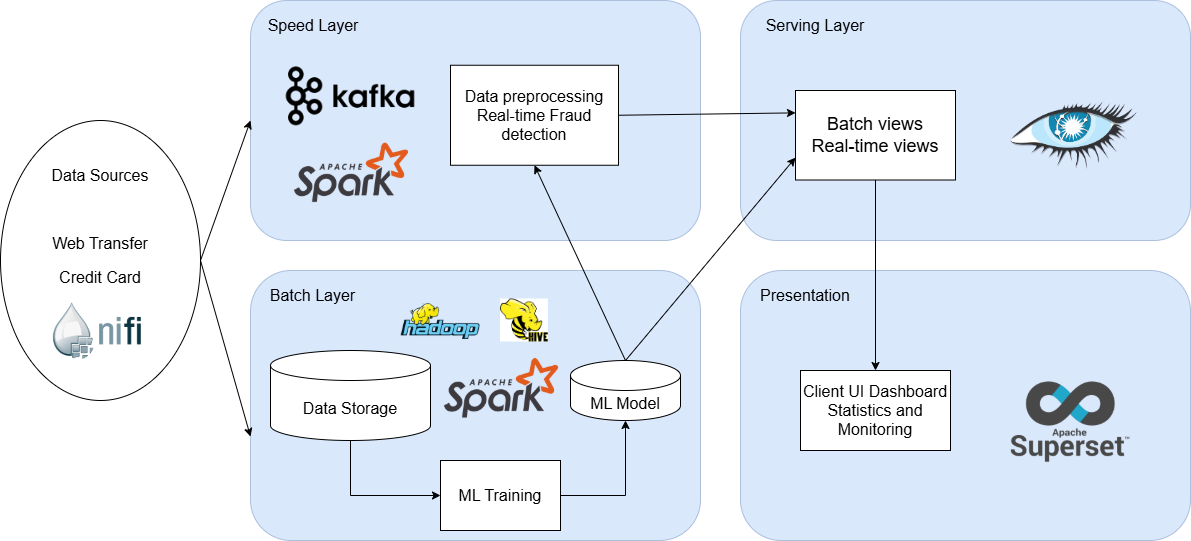
\includegraphics[width=0.95\textwidth]{images/m3-architecture.drawio.png}
    \caption{Project architecture}
    \label{fig:architecture}
\end{figure}

The following Big Data platforms will be used:
\begin{itemize}
    \item Apache NiFi: to collect and distribute the data from different sources;
    \item Apache Hadoop HDFS and Hive: as the main storage solution;
    \item Apache Cassandra as a view storage for fast querying;
    \item Apache Kafka: to work with the streaming data;
    \item Apache Spark: to make the batch processing and model training;
    \item Apache Superset: for data analysis on the user interface.
\end{itemize}

\section{Speed Layer}

The stream processing container is responsible for two main tasks: model training and message processing. 

At the moment, we have tested 4 models for fraud detection and selected Random Forest as it provided better performance on all of the datasets. A comparison of the model's performance is provided in the table below, including metrics precision (P) and recall (R).

\begin{table}[h!]
\centering
\begin{tabular}{|l|l|l|l|l|}
\hline
\textbf{}         & \textbf{LogisticRegression} & \textbf{GaussianNB} & \textbf{GradientBoosting} & \textbf{RandomForest} \\ \hline
\textbf{Dataset 1} & P: 0.35; R: 0.44           & P: 0.04; R: 0.18     & P: 0.9; R: 0.41           & \textbf{P: 0.97; R: 0.77}      \\ \hline
\textbf{Dataset 2} & P: 0.89; R: 0.58           & P: 0.79; R: 0.59     & P: 1.0; R: 0.99           & \textbf{P: 1.0; R: 0.99}       \\ \hline
\textbf{Dataset 3} & P: 0.0; R: 0.0             & P: 0.48; R: 0.1      & P: 1.0; R: 1.0            & \textbf{P: 1.0; R: 1.0}        \\ \hline
\end{tabular}
\caption{Performance metrics of fraud detection models}
\label{tab:metrics}
\end{table}

The initial model is being trained locally with a spark on the collected 'train' portion of the datasets.
As the next step, the streaming layer uses Spark Streaming in micro-batches mode to consume three Kafka streams and run predictions on them. Moreover, this module also includes the joining of these streams to produce additional insights.

\section{Batch Layer}

The batch layer is implemented using Apache Spark. On a regular basis (currently, every 5 minutes), the transaction data is taken from Hive to prepare some analytics on it. The resulting data is stored in Cassandra incrementally.

In particular, we are currently preparing data for the following views:
\begin{enumerate}
    \item Fraud Statistics by Transaction Type for the Dataset 1
    \begin{itemize}
        \item To analyze fraud patterns based on transaction types. We calculate fraud rates across specific transaction types to investigate whether certain types are more or less vulnerable to fraud.
    \end{itemize}
    \item Fraud Statistics by Transaction Amount for the Dataset 1
    \begin{itemize}
        \item To analyze fraud patterns based on transaction amounts. Similar to the previous view, the fraud rate is calculated, but across several amount ranges (0-1000, 1000-10000, 10000-50000, 50000-100000, 100000-500000, 500000+) instead of types.
    \end{itemize}
    \item Hourly Fraud Statistics for the Dataset 2
    \begin{itemize}
        \item To identify trends in fraudulent activities based on transaction hours. Given the timestamp of each transaction, we calculate the  amount of fraud as well as the percentage of fraud transactions per time frame (e.g., hour);
    \end{itemize}
    \item High-Risk Customer Analysis for the Dataset 2
    \begin{itemize}
        \item To identify customers with a high likelihood of fraud. The total amount of transactions per customer, as well as the fraud percentage, are calculated.
    \end{itemize}
\end{enumerate}



\section{Serving layer}

The serving layer relies on Apache Superset, TrinoDB, and Cassandra. Superset is an open-source data visualization and business intelligence platform well-suited for modern data pipelines due to its extensive support for a wide range of data sources and ease of integration into existing architectures.

\subsection{Integration of Apache Superset with the Current Architecture}
As illustrated in the architecture diagram:
\begin{itemize}
    \item The \textbf{Batch Layer}, powered by Apache Hive, processes large-scale data and aggregates it into queryable formats.
    \item The \textbf{Speed Layer}, which uses Kafka for real-time data ingestion and Spark for processing, produces real-time views stored in Cassandra. Superset can connect to Apache Cassandra through TrinoDB to display these real-time analytics, provided an appropriate connector is configured.
    \item The \textbf{Serving Layer} facilitates the querying of both batch and real-time views, making this data accessible to Superset for visualization in unified dashboards.
\end{itemize}

By integrating Superset with batch and speed layers, the system can provide users with comprehensive dashboards that include historical trends and real-time updates. This combination is particularly beneficial for monitoring critical use cases such as fraud detection, as it allows stakeholders to view both immediate alerts and long-term patterns.

\subsection{Advantages of Using Apache Superset}
\begin{itemize}
    \item \textbf{Ease of Use}: Superset provides an intuitive drag-and-drop interface for creating visualizations and dashboards, making it accessible to non-technical users.
    \item \textbf{Real-Time and Batch Data Integration}: Combining data from the speed and batch layers into unified dashboards enables comprehensive analytics and monitoring.
    \item \textbf{Custom Visualization}: Superset supports a variety of visualizations, allowing users to explore data in formats that best suit their needs, from basic bar charts to advanced geographic maps.
    \item \textbf{Scalability}: Being lightweight and web-based, Superset can handle a growing volume of data as the architecture scales.
    \item \textbf{Open Source and Extensibility}: Superset can be customized and extended to fit specific requirements as an open-source platform.
\end{itemize}

\subsection{Disadvantages and Challenges}
While Superset provides significant benefits, there are a few challenges and limitations to consider:
\begin{itemize}
    \item \textbf{Indirect Support for Kafka}: Superset does not natively connect to Kafka. Before it can be visualized, real-time data from Kafka must first be stored in a queryable data store (e.g., MongoDB or a similar OLAP engine).
    \item \textbf{Cassandra Support}: Superset does not have native support for Cassandra. Integration through a Python library or TrinoDB is required, adding some complexity.
    \item \textbf{Performance Considerations}: For real-time monitoring, performance can be a bottleneck if the underlying data stores are not optimized for frequent querying by Superset.
    \item \textbf{Learning Curve for Advanced Features}: While the primary interface is user-friendly, advanced configurations (e.g., complex filters and custom SQL queries) may require technical expertise.
\end{itemize}
The serving layer consists of two dashboards created in Apache Superset presented in Figure \ref{fig:batch-dashboard} and \ref{fig:speed-dashboard}. The dashboards present various charts created from the views generated by batch and streaming layers.


\begin{figure}[H]
    \centering
    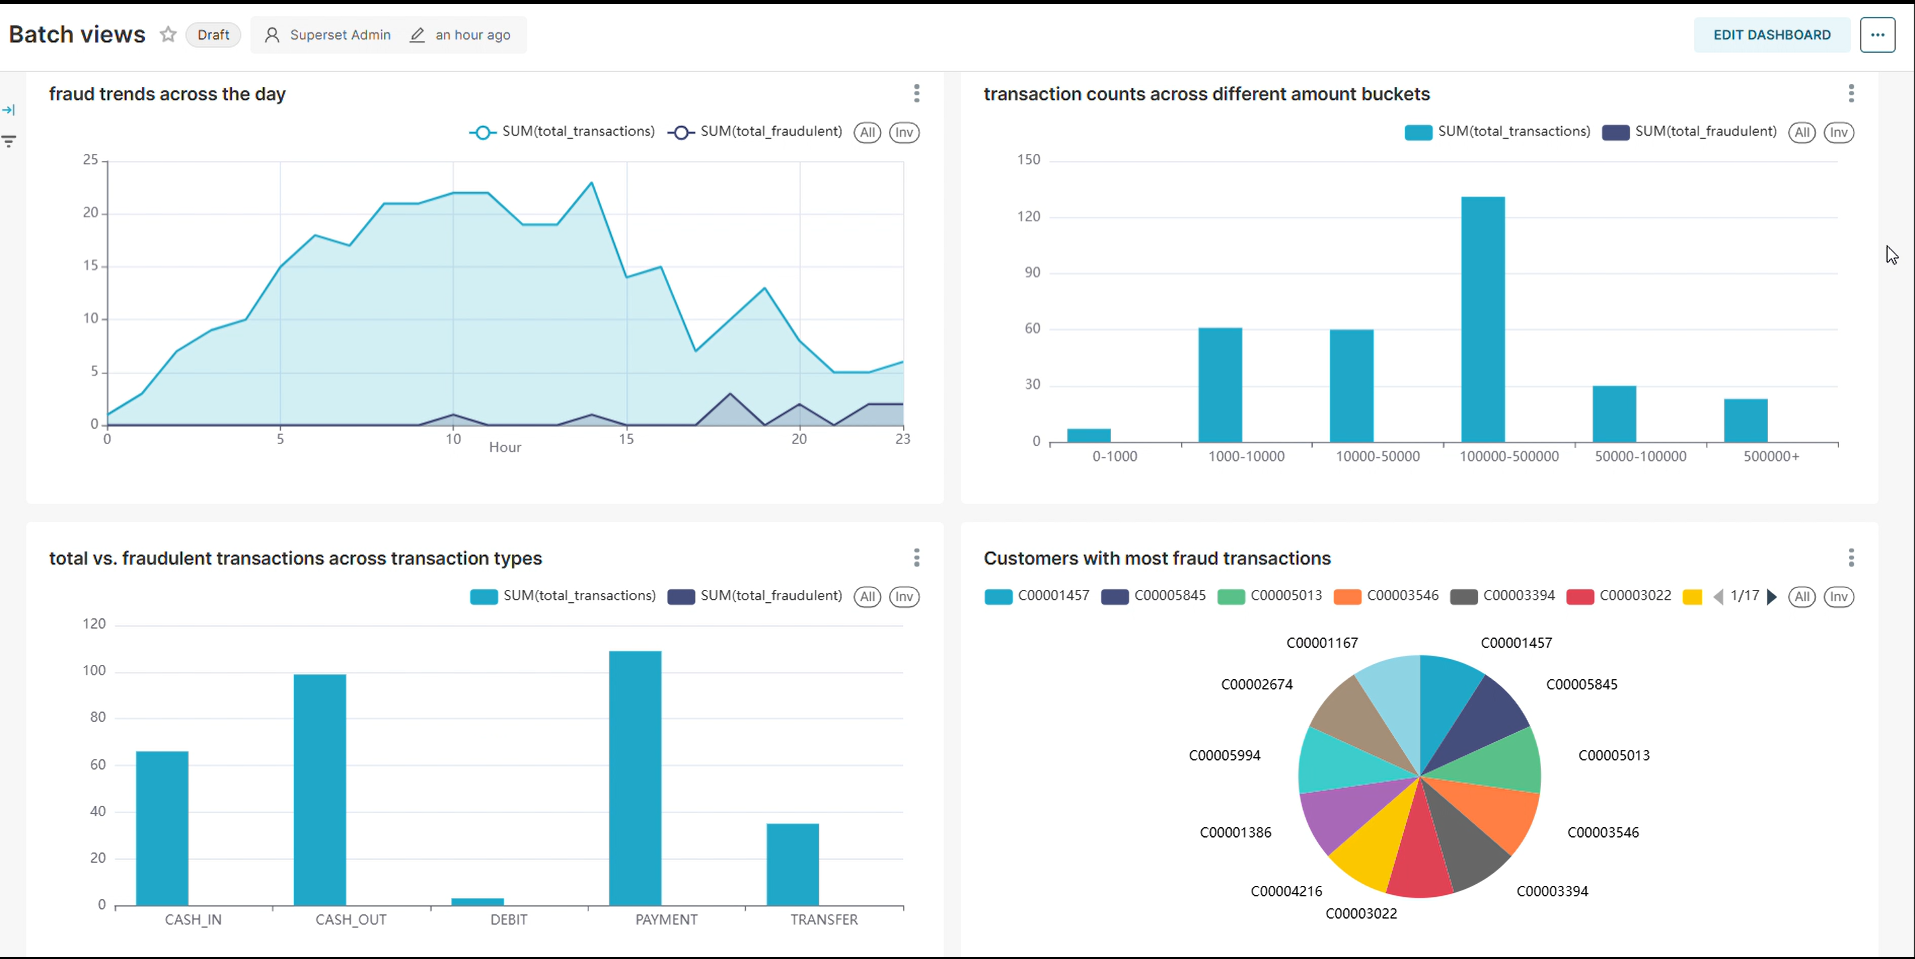
\includegraphics[width=0.95\textwidth]{images/superset-1.png}
    \caption{Batch layer dashboard}
    \label{fig:batch-dashboard}
\end{figure}


\begin{figure}[H]
    \centering
    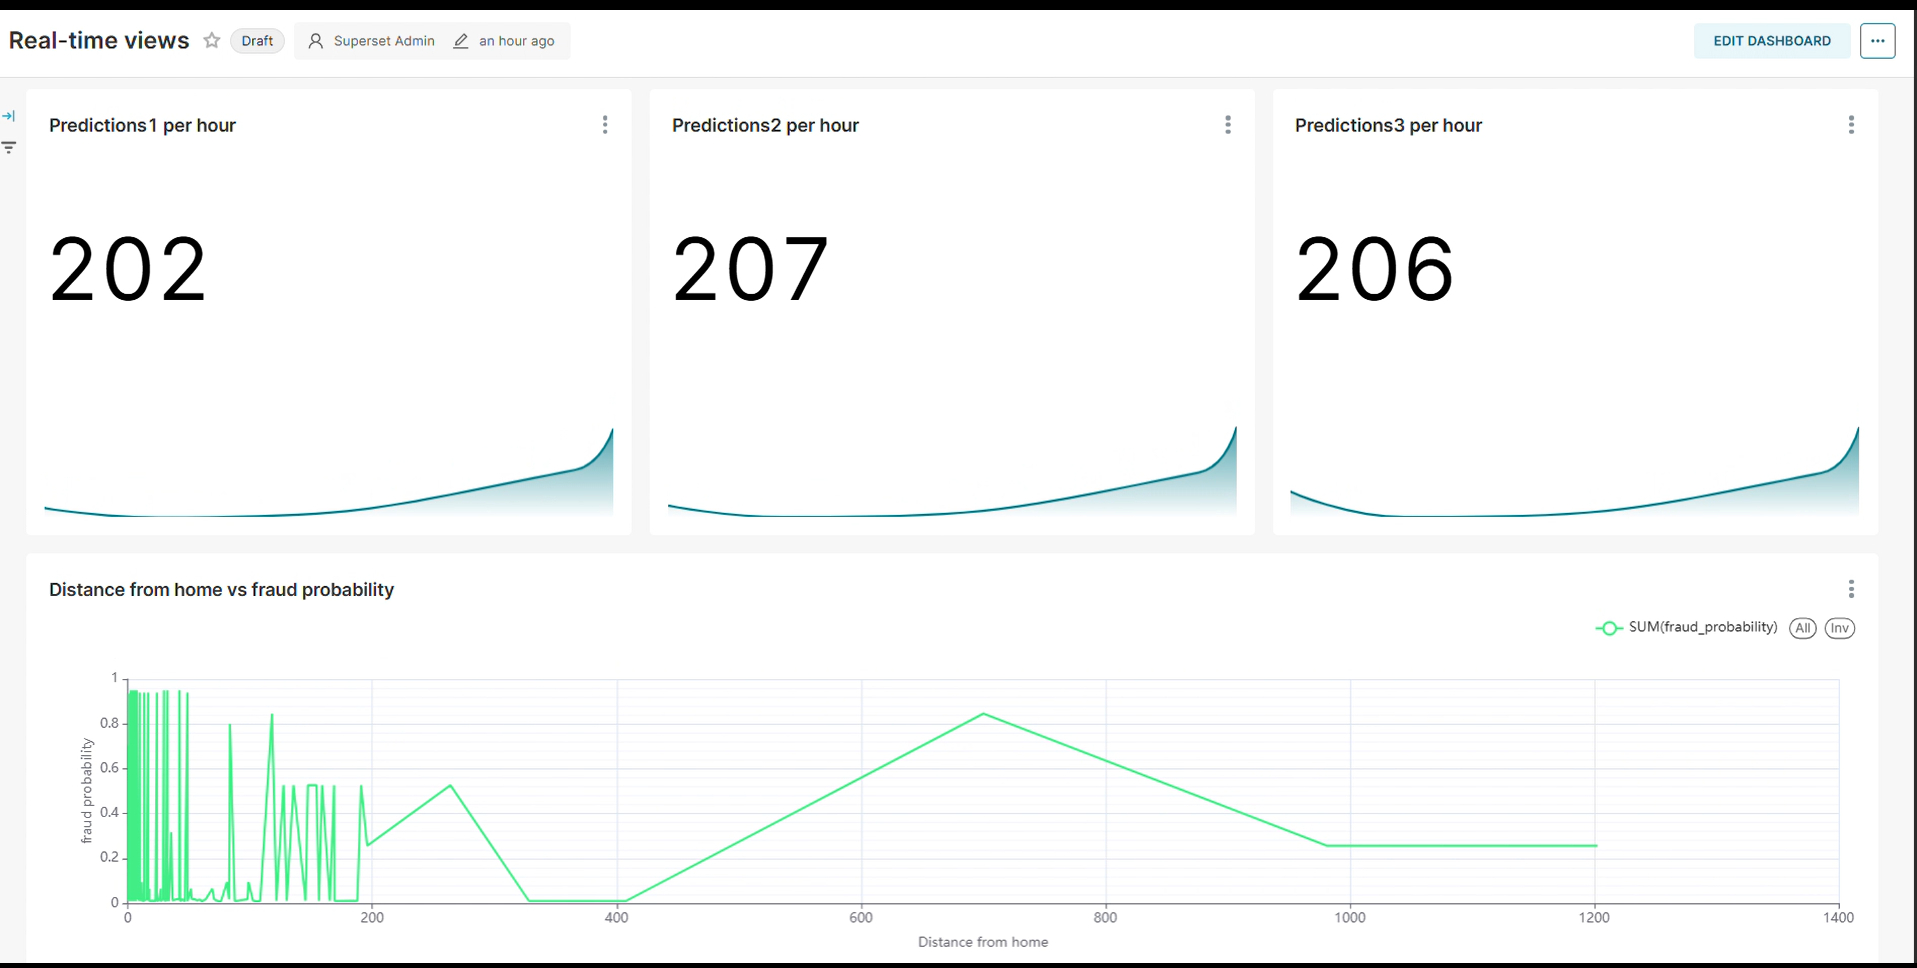
\includegraphics[width=0.95\textwidth]{images/superset-2.png}
    \caption{Speed layer dashboard}
    \label{fig:speed-dashboard}
\end{figure}

\section{Project impact}
The project of fraudulent transaction predictions has potential positive and negative impacts across various fields.
\begin{enumerate}
    \item Fraudulent transactions cost businesses and individuals billions annually. Detecting and preventing them minimizes these losses, protecting bottom lines and investor confidence.
    \item Reduced reliance on manual fraud assessment resulting in lower costs.
    \item Increased customer trust.
    \item Possibility to assist law enforcement in identifying and prosecuting fraudulent networks.
    \item Potential harm resulting from poor predictions.
    \item Some edge cases might have been missed, resulting in customer annoyance, such as false fraud predictions based on distance from the last transaction when going on holidays.
\end{enumerate}
The project has been realized with Big Data technologies, primarily based on Apache software and Docker, allowing for high fault tolerance and scalability. It is ready to handle incoming data robustly, representing the 5 Vs characteristics. However, for production-level quality, it should be extended with tools such as Kubernetes, allowing for seamless container scalability. It is worth pointing out that the whole system is resource expensive in regards to RAM, one needs to take that into consideration before planned deployment.

\section{Tasks assignment}

The table below contains the list of team members and the allocation of tasks to team members.

\begin{table}[htbp]
\centering
\begin{tabular}{|p{4cm}|p{6.5cm}|p{4cm}|}
\hline
\textbf{Team member} & \textbf{Tasks} & \textbf{Supporter} \\
\hline
Salveen Singh Dutt & Batch processing of the historical data for up-to-date model training (Batch Layer). & Karina Tiurina \\
\hline
Karina Tiurina & Fraud detection model training and fine-tuning; Data stream processing (Speed Layer). & Salveen Singh Dutt \\
\hline
Patryk Prusak & Data ingestion, collection, and preprocessing. & Karina Tiurina, Salveen Singh Dutt  \\
\hline
Patryk Prusak & Data visualization and configuration on the UI (Serving Layer). & Karina Tiurina, Salveen Singh Dutt \\
\hline
\end{tabular}
\caption{Tasks assignment}
\end{table}

\newpage

\begin{thebibliography}{9}

    \bibitem{dataset1}
    Chitwan Manchanda,
    \textit{Fraudulent Transactions Data},
    Kaggle, 2022.
    Available at: \url{https://www.kaggle.com/datasets/chitwanmanchanda/fraudulent-transactions-data}.
    
    \bibitem{dataset2}
    \textit{Credit\_Card\_Fraud\_},
    OpenML, 2024.
    Available at: \url{https://www.openml.org/search?type=data&status=active&id=45955&sort=runs}.

    \bibitem{dataset3}
    Carlos José,
    \textit{Credit Card Transactions Synthetic Data Generation},
    Kaggle, 2024.
    Available at: \url{https://www.kaggle.com/datasets/cgrodrigues/credit-card-transactions-synthetic-data-generation?select=transactions_df.csv}.
    
    \bibitem{dataset4}
    Machine Learning Group - ULB and Andrea,
    \textit{Credit Card Fraud Detection},
    Kaggle, 2018.
    Available at: \url{https://www.kaggle.com/datasets/mlg-ulb/creditcardfraud}.
    

    \bibitem{dataset4}
    \textit{Lambda Architecture},
    Cazton.
    Available at: \url{https://cazton.com/consulting/enterprise/lambda-architecture}.

    \bibitem{chatgpt}
    OpenAI,
    \textit{ChatGPT: Language Model},
    Available at: \url{https://chatgpt.com}.
    
    \end{thebibliography}


\end{document}